\chapter{Introduction to normal mixture models}





%% it 3
\section{Definitions}
\label{sec:def}

A good and thorough introductory book is the work of \cite{McL00} and
the reader is encouraged to study it to learn in depth about normal mixtures
and clustering. 
We will here give a short overview of normal mixtures to fix notation and 
nomenclature.
The motivating idea behind mixture models is, that in real world examples
a sample might be suspected to arise from more than one population or be 
more simply modelled by several overlayed distributions.
The example of this, that is generally considered to be the first of this kind,
is the one by Karl Pearson, who fitted two normal distributions with different 
means and variances.
In his book, \cite{Pea96}[Section 4.d.; page 266], Pearson analyzed measurements
of forehead to body length of crabs sampled from the bay of Naples. His mixture 
model-based approach suggested, that the crabs were evolving into two new 
subspecies.
This is a historically important example, because it presents statistical 
evidence of evolution in process.
%% the approach to decompose distributions has gained tremendous popularity after the availabity of computing power made parametrized MLE possible.
% TODO: fix sentence
Mixture models have been used since, but research took off after the 
availability of computing power made computational research possible
%TODO: less confused desc of pearsons research

% it 2
While the theory of mixture models holds for a much broader class of 
distributions, we restrict ourselves here to the case of normal distributions,
because this restriction fits more comfortably into the scope of this work and 
because normal distributions allow for a parsimonious parametrization, that is 
of interest to study.

% it 2
This parametrization is the $\pmb{LDL}\top$ decomposition, which allows a very 
simple parametrization and a straightforward connection between degrees of 
freedom and necessarily generated numerical values. This will be explained 
further in section \ref{sec:models}.

But before we delve deeper into the topic of this research, we first define the
concept of a normal mixture model:

Let $ \mu \in \mathbb{R}^p , \quad \Sigma \in \mathbb{R}^{p \times p} $ be
symmetric positive definite and $ \phi(- ; \mu, \Sigma) $ be the normal 
distribution with mean $ \mu $ and covariance matrix $ \Sigma $ with density 
function:

\begin{equation} 
    \phi(\pmb{x;\mu,\Sigma})=
    \frac{\exp(-\frac{1}{2}(\pmb{x-\mu})\pmb{\Sigma}^{-\frac{1}{2}}(\pmb{x-\mu})^\top)}
         {\sqrt{(2\pi)^k \det{\pmb{\Sigma}}}}  
\end{equation}

for $\pmb{x} \in \mathbb{R}^p$.
Since we are studying mixture models, we will need several overlapping of 
normal distributions, of differing means and covariance. Therefore, we choose
notation allowing us to refer to the components in shorthand. Let us assume we
have $K \in \mathbb{N}$ normal distributions with means and covariance 
$\pmb{\mu}_k, \pmb{\Sigma}_k,\quad k \in \{1, \dots , K\}$, then we fix:

\begin{equation} 
    \phi_k(\pmb{x}) := \phi(\pmb{x;\mu_k, \Sigma_k})
    \label{eqn:phik}
\end{equation}

And going forward, we will refer to components by the subscript $k$.


\begin{definition}
    Suppose we have a random sample $ \pmb{Y}_1, \dots , \pmb{Y}_n $, where
    $\pmb{Y}_i$ is a $p$-dimensional random vector with probability density 
    function $ \pmb{Y}_i \sim f(\pmb{y}_i) $ on $\mathbb{R}^p$.

    We assume that the density $ f(\pmb{y}_i) $ of $ \pmb{Y}_i $ can 
    be written in the form: 
    \begin{equation} 
        f(\pmb{y}_i) = \sum_{k=1}^{K} \pi_k \phi_k (\pmb{y}_i)
        \label{eqn:mixture}
    \end{equation}
    The $\phi_k$ are normal distributions and are called the mixture components
    with parameters $\pmb{\mu}_k$ and $\pmb{\Sigma}_k$ as described above 
    (\ref{eqn:phik}).
    The $ \pi_k $ are called the component densities of the mixture and are
    constrainded by the rules $\pi_k > 0$ and $\sum_k \pi_k = 1$.

\end{definition}

%TODO: need some fill text here?

% it 1
For 'large' datasets there are more parsimonious parametrizations, that reduce
computation time. These, for example, assume that all components have the same
covariance, or have certain restrictions placed on them. We will give a 
detailed description of the models assumed in this thesis in section 
\ref{sec:models}.


\section{The EM-Algorithm in Sketch}
\label{sec:sketch}

%% it 1
With this definition, we immediately face the problem of how to fit these
mixture components to given data. A popular algorithm to solve this problem 
is the {\bf E}xpectation-{\bf M}aximization algorithm, abbreviated as 
EM-algorithm.

We give here a sketch of the EM-algorithm in the case of all normal mixture 
components. This roughly follows the content in \cite{McL00}. For a more 
thorough treatment of the matter see chapter 3.

Suppose we have a $p-$dimensional dataset of $n$ samples $x_1, \dots ,x_n$,
onto which we would like to fit a $K$ component normal mixture with mixture
components $\phi_k,\ k \in {1,\dots , n}$. 

For the EM-algorithm further parameters are introduced. These are denoted
$\tau_j(\pmb{y}_i)$ and they represent the posterior probabilities that 
observation $i$ is a member of component $j$.

The EM-algorithm is a two step, iterative process consisting of an 'e'-step
and an 'm'-step.
In the e-step the expectation of component membership is updated.
\begin{equation} 
    \tau_j(\pmb{y}_i;\Psi) = \phi_j(\pmb{y}_i)/ \sum_{k=1}^K \phi_k(\pmb{y}_i)
\end{equation}
and in the m-step given the component membership information we update the 
component means and covariances by weighted versions of the usual estimators.
\begin{equation}
    \pmb{\mu}_j = \sum_{i=1}^n \tau_j(\pmb{y}_i)\pmb{y}_i / \sum_{j=1}^n \tau_j(\pmb{y}_i)
\end{equation}
\begin{equation}
    \pmb{\Sigma}_j = \sum_{i=1}^n \tau_j(\pmb{y}_i) (\pmb{y}_i- \pmb{\mu}_j)(\pmb{y}_i-\pmb{\mu}_j)^\top /  \sum_{i=1}^n \tau_j(\pmb{y}_i)
\end{equation}


% it 2
There remains to be stated how to start the algorithm. Since both steps of the
algorithm depend on data from the other, the EM-algorithm needs some form of 
initialization step.
Most popular implementations use some form of pre clustering and use the 
EM-algorithm as subsequent tools to fit the data. The R-package {\tt mclust} 
for example uses hierarchical agglomerative clustering \cite{Scr16}.

% TODO: some fluff text here


\section{Choice of Notation}
\label{sec:notation}

% it 1
The classification of models in this paper relies heavily on the work of 
\cite{Cel95}, however, out of necessity for clarity, we break with their 
notation. 
So as to not confuse the reader we describe here in depth the differences in 
notation between \cite{Cel95} and ours.

The basis of classification in \cite{Cel95} is the decomposition of a
symmetric matrix into an orthogonal and a diagonal component.
A symmetric positive definite matrix $ \Sigma $ can be decomposed as follows
\begin{equation} 
    \Sigma = \lambda \pmb{D} \pmb{A} \pmb{D}^{\top}
\end{equation}
with $ \pmb{D} $ an orthogonal matrix and $ \pmb{A} $ a diagonal matrix and
$ \lambda = \sqrt[\uproot{3}p]{det(\Sigma)} $ the $ p-th $ root of the 
determinant of $ \Sigma $.

This decomposition has an appealing geometric interpretation, with $ \pmb{D} $ 
as the \textit{orientation} of the distribution, $ \pmb{A} $ the \textit{shape},
and $ \lambda $ the \textit{volume}. The problem of notation comes from standard 
conventions in linear algebra, where the letters $A$ and $D$ are usually 
occupied by arbitrary and diagonal matrices respectively. Furthermore, we intend
to apply a variant of the Cholesky decomposition to $ \Sigma $, the 
$ \alpha\pmb{L}\pmb{D}\pmb{L}^{\top} $ decomposition. This obviously raises some
conflicts in notation.

Therefore we, from here on, when referring to the decomposition as described by 
\cite{Cel95}, will use the following modification of notation:

\begin{gather} 
    \pmb{D} \longmapsto \pmb{Q} \\
    \pmb{A} \longmapsto \pmb{\Lambda} \\
    \lambda \longmapsto \alpha  \\
    \Sigma = \lambda \pmb{D} \pmb{A} \pmb{D}^\top =
        \alpha \pmb{Q} \pmb{\Lambda} \pmb{Q}^\top
\end{gather}

These were chosen according to general conventions of linear algebra. $ \pmb{Q} $
is usually chosen for orthonormal matrices; $ \pmb{\Lambda} $ is often a choice 
for diagonal matrices of eigenvectors and $ \alpha $ was somewhat arbitrarily 
chosen.


\section{Models of Covariance Matrices}
\label{sec:models}


% it 1
As mentioned above, there are ways to constrain the covariance matrices for 
computational reasons. There are istances where the resulting loss of 
information is seen as acceptable, for example if, through consideration of the
data, that a simplified model is acceptable. Another is if the sheer size of 
the data makes application of full generality impossible.
\begin{itemize}
    \item We restrict the complexity of the decomposition components
    \item We restrict the variability of the mixture components
\end{itemize}
Let us look at the first case. We take the decomposition of a covariance matrix
as $\Sigma = \alpha \pmb{Q\Lambda Q}^\top$. Of these, we can simplify the 
structure of $\pmb{Q}$ and $\pmb{\Lambda}$, by replacing them with the identity.
If we set $\pmb{Q}=\mathrm{Id}$, we lose the freedom of orientation and if we 
set $\pmb{\Lambda}=\mathrm{Id}$ we restrict ourselves to spherical 
distributions.

of course, we cannot restrict $\pmb{\lambda}$ while letting $\pmb{q}$ free, 
since
\begin{equation} 
    \pmb{Q\Lambda Q}^\top = \pmb{Q}\mathrm{Id}\pmb{Q}^\top = \mathrm{Id}
\end{equation}

The second restriction simply means we hold the decomposition fixed throughout 
all covariance matrices.
% it 1
There is however an issue with the cholesky decomposition. For 10 out of 14
cases as defined by \cite{Cel95}, there exists a canonical translation of
decompositions.
The 6 diagonal cases need no translation; the eigen and cholesky decomposition
are equal to identity.
For the non-diagonal cases note that for a given sym. pos. def. matrix
$ \Sigma $ we have decompositions:
\begin{equation}
    \Sigma = \alpha \pmb{Q \Lambda Q}^\top \quad \Sigma =\alpha \pmb{L D L}^\top
\end{equation}
Since in both cases the enclosing matrices $ \pmb{Q} $ and $ \pmb{L} $ have 
determinant $ 1 $ the determinant of $ \Sigma $ falls entirely on $ \alpha $.
therefore $ \alpha $, in these particular decompositions, is equal for both.
\cite{Cel95} vary $\sigma$ by either varying or holding fixed the volume 
$(\alpha / \alpha_k)$, shape $(\pmb{\Lambda} / \pmb{\Lambda_k})$ and orientation
$(\pmb{Q} / \pmb{Q}_k)$.
These 3 times 2 cases would yield the 8 out of 14 cases of non-diagonal cases.
However there is no canonical transform for either variable orientation and 
fixed shape or fixed orientation and variable shape.
The reason for this is that in the $\pmb{LDL}^\top$ decomposition the lower
diagonal matrix $\pmb{L}$ holds some of the shape of the matrix, which in 
the eigendecomposition is in the $\pmb{\Lambda}$ matrix.
In fact, $\pmb{L}$ is orthogonal if and only if 
$\pmb{L} = \mathrm{Id}_{n\times n}$.
Therefore we can only decompose matrices where either both or neither shape and
orientation vary. See table \ref{table:paramSigma}.

While we could in theory construct the cases $\pmb{L}\pmb{D}_k\pmb{L}^\top$ and
$\pmb{L}_k \pmb{D} \pmb{L}_k^\top$, however they do not correspond to the desired
geometric intent behind the differentiation of models and are therefore not 
included.


\begin{table}[!htb]
    \centering
    \rotatebox{90}
    {
        \begin{tabular}{| c | c c c c c | c c c |}
            \hline
            Model & $\pmb{\Sigma}_k$ C\&G & volume & shape & orientation & parameters & $ \pmb{LDL}^\top $ & parameters & count \\
            \hline

            EII    & $ \alpha \pmb{I} $ & equal & equal & - & $ \alpha $ & as in C\&G & & 1 \\
            VII    & $ \alpha_k \pmb{I} $         & var. & equal & - & $ \alpha_k $ & & & $K$  \\
            EEI    & $ \alpha \pmb{\Lambda} $     & equal & equal & coord. axes & $ \alpha, \lambda_i $ & & & $ 1+(p-1) $\\
            VEI    & $ \alpha_k \pmb{\Lambda} $ & var. & equal & coord. axes & $ \alpha_k, \lambda_{i}$ & & & $ K+(p-1) $ \\
            EVI    & $ \alpha \pmb{\Lambda}_k $ &equal & var. & coord. axes & $ \alpha, \lambda_{i,k} $ & & & $ 1+K(p-1) $ \\
            VVI    & $ \alpha_k \pmb{\Lambda}_k $ & var. & var. & coord. axes & $ \alpha_k, \lambda_{i,k} $ & & & $ K+K(p-1) $ \\
            \hline
            EEE    & $ \alpha \pmb{Q \Lambda Q}^\top $ &equal & equal & equal & $ \alpha, \lambda_{i}, q_{i,j} $ & $ \alpha \pmb{LDL}^{\top} $ & $ \lambda , d_i, l_{i,j} $ & $ 1+(p-1)+\frac{p(p-1)}{2} $ \\
            \hline
            EVE    & $ \alpha \pmb{Q \Lambda}_k \pmb{Q}^\top $ &equal & var. & equal & $ \alpha, \lambda_{i,k}, q_{i,j} $  & doesn't exist & & $ 1+K(p-1)+\frac{p(p-1)}{2} $ \\
            \hline
            VEE    & $ \alpha_k \pmb{Q \Lambda Q}^\top $ & var. & equal & equal & $ \alpha_k, \lambda_{i}, q_{i,j} $ & $ \alpha_k \pmb{LDL}^\top $ & $ \lambda_k , d_i, l_{i,j} $ & $ K+(p-1)+\frac{p(p-1)}{2} $ \\
            \hline
            VVE    & $ \alpha_k \pmb{Q \Lambda}_k \pmb{Q}^\top $ &var. & var. & equal & $ \alpha_k, \lambda_{i,k}, q_{i,j} $ & & & $ K+K(p-1)+\frac{p(p-1)}{2} $ \\
            EEV    & $ \alpha \pmb{Q}_k \pmb{\Lambda} \pmb{Q}_k^\top $ &equal & equal & var. & $ \alpha, \lambda_{i}, q_{i,j,k} $ &  don't exist  & & $ 1+(p-1)+K\frac{p(p-1)}{2} $ \\
            VEV    & $ \alpha_k \pmb{Q}_k \pmb{\Lambda} \pmb{Q}_k^\top $ &var. & equal & var. & $ \alpha_k, \lambda_{i}, q_{i,j,k} $ & & & $ K+(p-1)+K\frac{p(p-1)}{2} $ \\
            \hline
            EVV    & $ \alpha \pmb{Q}_k \pmb{\Lambda}_k \pmb{Q}_k^\top $ & equal & var. & var. & $ \alpha, \lambda_{i}, q_{i,j,k} $ & $ \alpha \pmb{L}_k \pmb{D}_k \pmb{L}_k^\top $ & $ \lambda, d_{i,k}, l_{i,j,k}\ j>i $ & $ 1+K(p-1)+K\frac{p(p-1)}{2} $  \\
            VVV    & $ \alpha_k \pmb{Q}_k \pmb{\Lambda}_k \pmb{Q}_k^\top $ & var. & var. & var. & $ \alpha_k, \lambda_{i}, q_{i,j,k} $ & $ \alpha_k \pmb{L}_k \pmb{D}_k \pmb{L}_k^\top $ & $ \lambda_k, d_{i,k}, l_{i,j,k}\ j>i $ & $ K+K(p-1)+K\frac{p(p-1)}{2} $ \\
            \hline
        \end{tabular}
    }
    \caption{Table of Parameters of the Covariance Matrices}
    \label{table:paramSigma}
\end{table}

\clearpage

%% TODO: fluff text, connecting the two tables
\begin{table}
    \centering
    \begin{tabular}{l|l l|l|r}
        $\Sigma$ model  & $\mu$, $\pi$  & $\Sigma$      & total \#\{par\}       & $\mathcal{O}()$ \\
        \hline
        EII        & $ K -1 + pK$  & $1$                        & $Kp+K$                & $Kp$ \\
        VII        & $ K -1 + pK$  & $K$                        & $Kp+2K-1$             & $Kp$ \\
        EEI        & $ K -1 + pK$  & $1+(p-1)$                  & $Kp+p+K-1$            & $Kp$ \\
        VEI        & $ K -1 + pK$  & $K+(p-1)$                  & $Kp+p+2K-2$           & $Kp$ \\
        EVI        & $ K -1 + pK$  & $1+K(p-1)$                 & $2Kp$                 & $Kp$ \\
        VVI        & $ K -1 + pK$  & $K+K(p-1)$                 & $2Kp+K-1$             & $Kp$ \\
        EEE        & $ K -1 + pK$  & $1+(p-1)+\frac{p(p-1)}{2}$         & $\frac{(p+2)(p-1)}{2}+Kp+K$    
            & $p^2+Kp$ \\
        VEE        & $ K -1 + pK$  & $K+(p-1)+\frac{p(p-1)}{2}$         & $\frac{(p+2)(p-1)}{2}+Kp+2K-2$  
            & $p^2+Kp$ \\
        EVV        & $ K -1 + pK$  & $1+K(p-1)+K\frac{p(p-1)}{2}$       & $K\frac{(p+2)(p-1)}{2}+Kp+K$       
            & $Kp^2$ \\
        VVV        & $ K -1 + pK$  & $K+K(p-1)+K\frac{p(p-1)}{2}$       & $K\frac{(p+2)(p-1)}{2}+Kp+2K-1$       
            & $Kp^2$ \\
    \end{tabular}
    \caption{Full Table of Parameters}
    \label{table:param}
\end{table}

%% here explain why ldlt is so nice to parametrize; i.e. Q in QLambdaQt has as many
%% degrees of freedom, but needs more complicated boundary conditions to work well.
% it 1
There is an attractive advantage in using the $\pmb{LDL}^\top$ decomposition.
Since both the $\pmb{LDL}^\top$ and eigendecomposition derive from the same 
covariance matrix, the necessary parameters are the same in cardinality.
In the case of the $\pmb{Q}$ and $\pmb{L}$ matrices, there need to be $\frac{p(p-1)}{2}$
parameters to be determined to uniquely define these matrices.
In the case of the $\pmb{L}$ matrix these are straightforward the entries of 
the lower diagonal matrix, whereas $\pmb{Q}$ needs a nontrivial amount of work
to determine a minimal generating set of parameters, which makes computation
of the decomposition as in \cite{Cel95} a lot more difficult.
Therefore the $\pmb{LDL}^\top$ decomposition was chosen for the purpose of this
thesis.


\section{Problems of the EM-algorithm}
\label{sec:emproblems}


The EM-algorithm has stalling problems especially close to a local optimum.
% it 1
In their seminal work, \cite{Dem77}, have proven that the EM-algorithm 
converges under mild regularity conditions. 
%TODO: talk more about Dem77, in more detail about convergence conditions
However, convergence does not guarantee fast convergence. In fact, a lot of 
the work, that has gone into the research around the EM-algorithm has been 
concerned with speeding up convergence, see \cite{McL00}[section 2.17].
The concern here is that a slowing in convergence might be mistaken for actual
convergence.

% it 1
This phenomenon is not infrequent and in difficult mixtures quite visible.
To illustrate let us look at a particular mixture taken from \cite{Mar92} and
the {\tt nor1mix} package from CRAN.
{\tt nor1mix} is a package designed and developed for educational purposes to 
teach about univariate normal mixtures. It is also the spiritual predecessor 
of this thesis' \Rp code.

The mixture is a trimodal mixture of uneven weight, as shown in figure
\ref{fig:MW.nm9}.
While not the most difficult mixture studied by \cite{Mar92}, it is certainly
not trivial either.
In the figures below, \ref{fig:20em} and \ref{fig:200em}, we demonstrate, that
even after 200 iterations of the EM-algorithm the convergence is poor.
In this instance, the initialization is done using \Rp's CLARA implementation
from the cluster package. %TODO: citation here.



\begin{figure}[h]
    \centering
    \begin{minipage}{0.45\textwidth}
\begin{Schunk}
\begin{Sinput}
>     library("nor1mix")
>     MW.nm9 ## Trimodal mixture
\end{Sinput}
\begin{Soutput}
'Normal Mixture' object 	 ``#9 Trimodal'' 
       mu sigma    w
[1,] -1.2  0.60 0.45
[2,]  1.2  0.60 0.45
[3,]  0.0  0.25 0.10
\end{Soutput}
\end{Schunk}
% TODO: fix position size??
        \caption{Parameters of {\tt MW.nm9}}
        \label{tab:MW.nm9}
    \end{minipage}
    \begin{minipage}{0.45\textwidth}
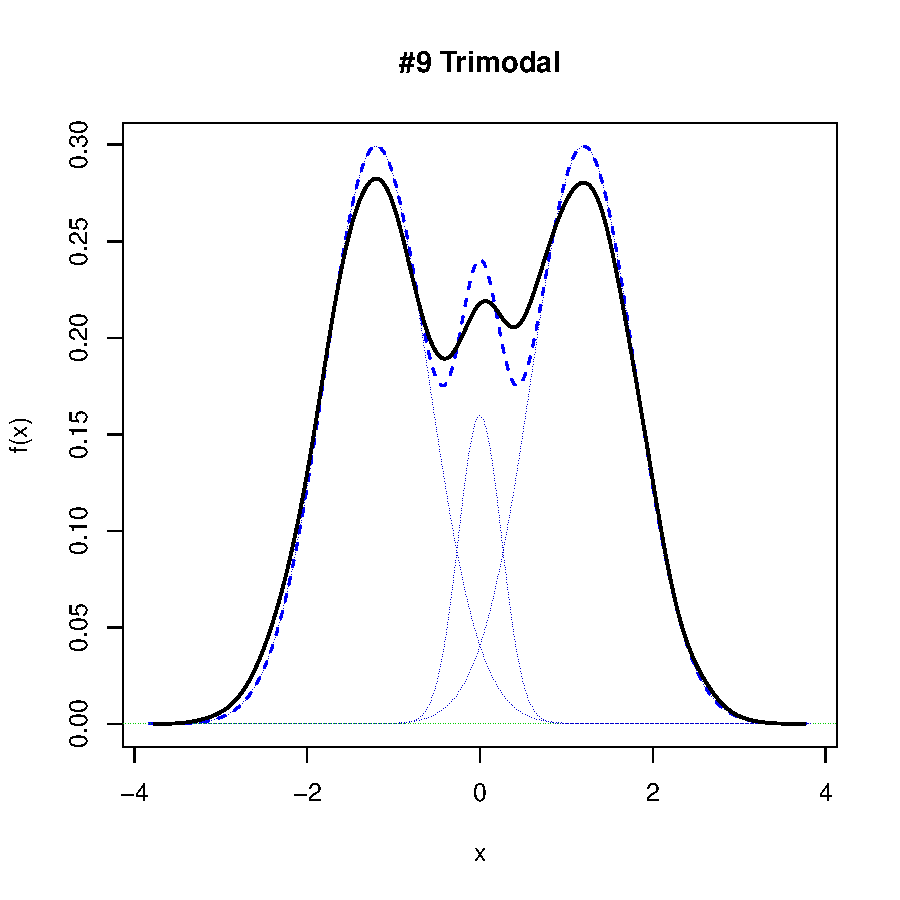
\includegraphics{chapter1-figTrimodal}
        \caption{True and Estimated density}
        \label{fig:MW.nm9}
    \end{minipage}
\end{figure}
% TODO: fix placement issue and caption location

then an illustration of MW examples of pathological cases

We can see, that the EM-algorithm seems to converge to an intermediary
solution, where the smaller middle solution is weighted lower, until it manages
to correct back and find the correct components.





\begin{figure}[h]
    \centering
    \begin{minipage}{0.45\textwidth}
    \centering
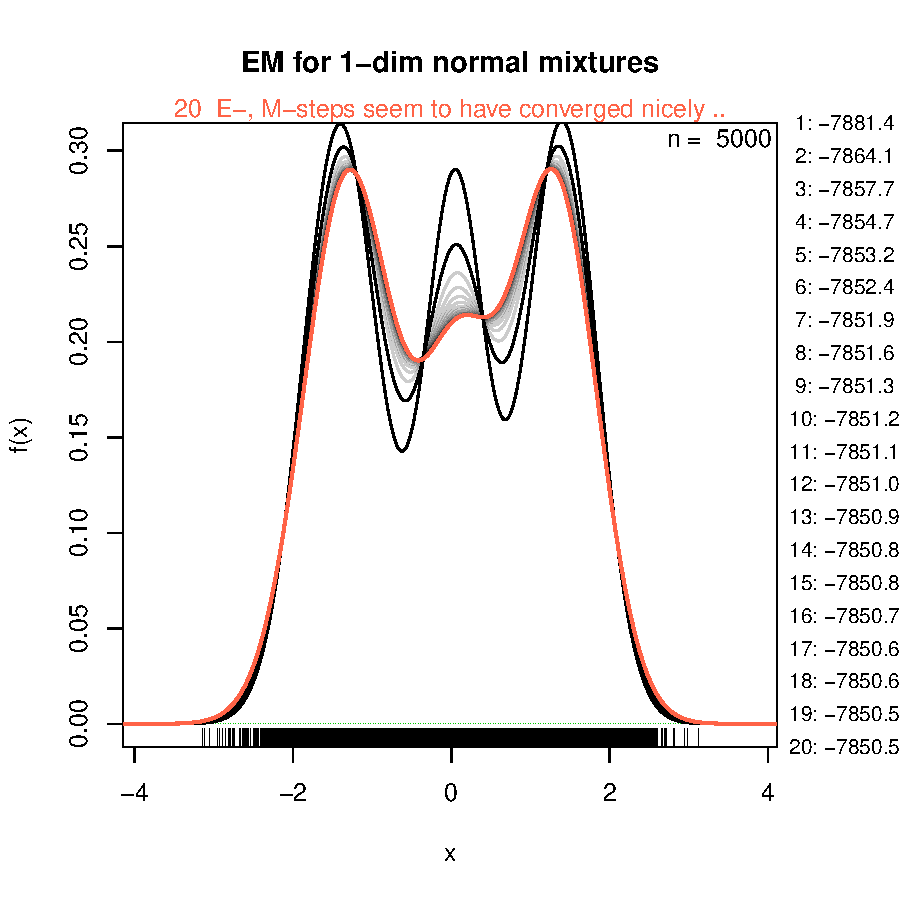
\includegraphics{chapter1-fignor1mixEx}
    \label{fig:20em}
    \caption{20 EM steps}
    \end{minipage}\hfill
    \begin{minipage}{0.45\textwidth}
    \centering
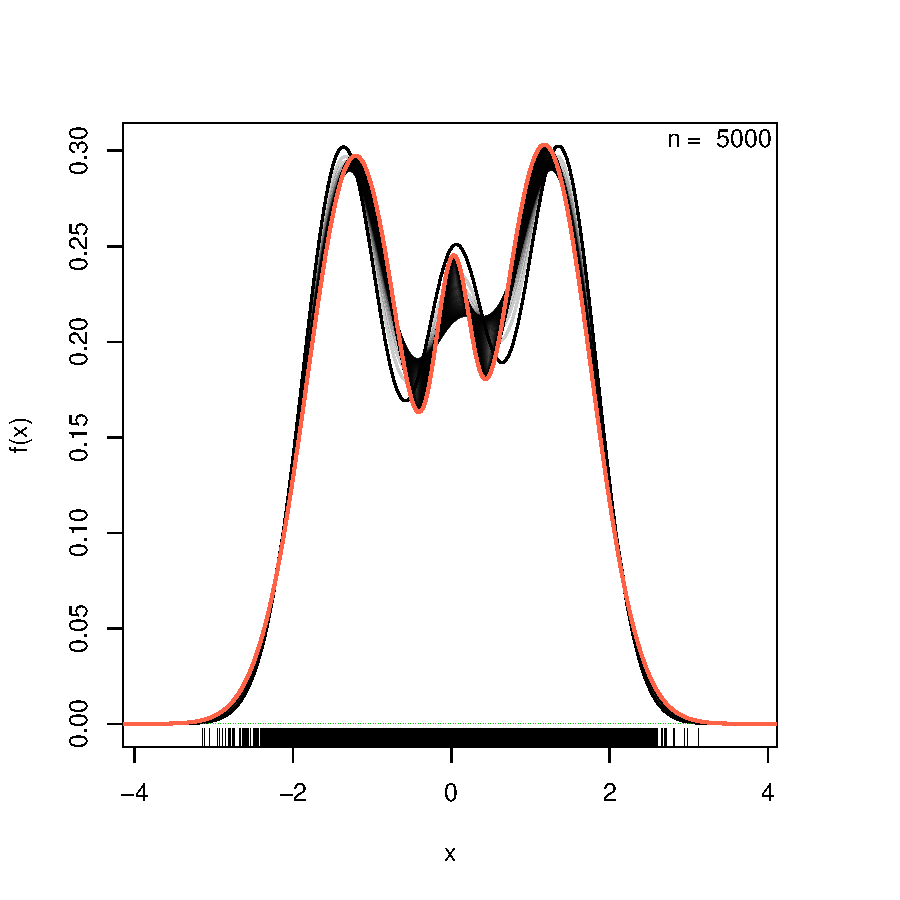
\includegraphics{chapter1-figplotemsteps}
    \label{fig:200em}
    \caption{200 EM steps}
    \end{minipage}
    \label{adfafdafds}
\end{figure}

We see how change in log-likelihood seems to stagnate. However, this does not 
stay that way. If we let EM run a bit further we see, the log-likelihood hits 
a flatspot, after which convergence accelerates again.


\begin{figure}[h]
    \centering
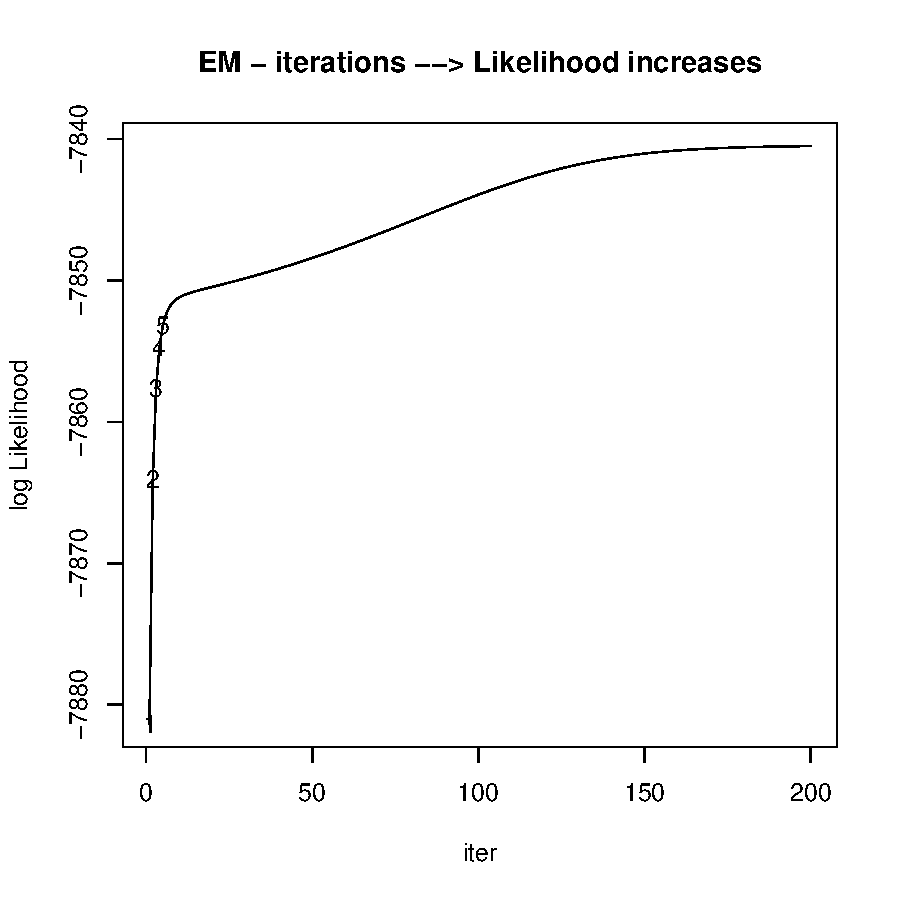
\includegraphics{chapter1-figemll}
    \label{fig:emll}
    \caption{Log-likelihood Plotted against Iteration Count for the Example in \ref{fig:200em}}
\end{figure}



In fact, it seems that the previous solution is a saddle point in the likelihood
function, where EM has chronic problems continuing improvements.

give 2D demonstration.


\section{Alternative Option}
\label{sec:alt}


% it 1
In conclusion, the EM-algorithm has very appealing advantages. However, as we
have shown, there are chronic problems in convergence rates. The aim of this 
thesis is to test if some improvement could be achieved by a different method.

The plan is reasonably straightforward:

\begin{enumerate}
    \item Initialize using CLARA.
    \item Perform one m-step, to transform CLARA's results into the form of a 
        normal mixture.
    \item Apply a general optimizer, using the mixture's log-likelihood function.
\end{enumerate}

%% this is going to be a longer part

% TODO: here need fluff text explaining motivation of package
what do we hope from this?
better convergence
proof of concept i.e. not complete failure

raise questions about implementation,
clara fctn
optim params

the subsequent chapter is devoted to answering this question by documenting the 
development of norMmix


%% TODO: need somwhere that MLE is abbreviated ...
